\PassOptionsToPackage{unicode=true}{hyperref} % options for packages loaded elsewhere
\PassOptionsToPackage{hyphens}{url}
%
\documentclass[
  ignorenonframetext,
]{beamer}
\usepackage{pgfpages}
\setbeamertemplate{caption}[numbered]
\setbeamertemplate{caption label separator}{: }
\setbeamercolor{caption name}{fg=normal text.fg}
\beamertemplatenavigationsymbolsempty
% Prevent slide breaks in the middle of a paragraph:
\widowpenalties 1 10000
\raggedbottom
\setbeamertemplate{part page}{
  \centering
  \begin{beamercolorbox}[sep=16pt,center]{part title}
    \usebeamerfont{part title}\insertpart\par
  \end{beamercolorbox}
}
\setbeamertemplate{section page}{
  \centering
  \begin{beamercolorbox}[sep=12pt,center]{part title}
    \usebeamerfont{section title}\insertsection\par
  \end{beamercolorbox}
}
\setbeamertemplate{subsection page}{
  \centering
  \begin{beamercolorbox}[sep=8pt,center]{part title}
    \usebeamerfont{subsection title}\insertsubsection\par
  \end{beamercolorbox}
}
\AtBeginPart{
  \frame{\partpage}
}
\AtBeginSection{
  \ifbibliography
  \else
    \frame{\sectionpage}
  \fi
}
\AtBeginSubsection{
  \frame{\subsectionpage}
}
\usepackage{lmodern}
\usepackage{amssymb,amsmath}
\usepackage{ifxetex,ifluatex}
\ifnum 0\ifxetex 1\fi\ifluatex 1\fi=0 % if pdftex
  \usepackage[T1]{fontenc}
  \usepackage[utf8]{inputenc}
  \usepackage{textcomp} % provides euro and other symbols
\else % if luatex or xelatex
  \usepackage{unicode-math}
  \defaultfontfeatures{Scale=MatchLowercase}
  \defaultfontfeatures[\rmfamily]{Ligatures=TeX,Scale=1}
\fi
\usetheme[]{AnnArbor}
\usecolortheme{dolphin}
\usefonttheme{structurebold}
% use upquote if available, for straight quotes in verbatim environments
\IfFileExists{upquote.sty}{\usepackage{upquote}}{}
\IfFileExists{microtype.sty}{% use microtype if available
  \usepackage[]{microtype}
  \UseMicrotypeSet[protrusion]{basicmath} % disable protrusion for tt fonts
}{}
\makeatletter
\@ifundefined{KOMAClassName}{% if non-KOMA class
  \IfFileExists{parskip.sty}{%
    \usepackage{parskip}
  }{% else
    \setlength{\parindent}{0pt}
    \setlength{\parskip}{6pt plus 2pt minus 1pt}}
}{% if KOMA class
  \KOMAoptions{parskip=half}}
\makeatother
\usepackage{xcolor}
\IfFileExists{xurl.sty}{\usepackage{xurl}}{} % add URL line breaks if available
\IfFileExists{bookmark.sty}{\usepackage{bookmark}}{\usepackage{hyperref}}
\hypersetup{
  pdftitle={Docker: o que é e para que serve},
  pdfauthor={Luiz Sol e Marcos Vinicius},
  pdfborder={0 0 0},
  breaklinks=true}
\urlstyle{same}  % don't use monospace font for urls
\newif\ifbibliography
\usepackage{color}
\usepackage{fancyvrb}
\newcommand{\VerbBar}{|}
\newcommand{\VERB}{\Verb[commandchars=\\\{\}]}
\DefineVerbatimEnvironment{Highlighting}{Verbatim}{commandchars=\\\{\}}
% Add ',fontsize=\small' for more characters per line
\usepackage{framed}
\definecolor{shadecolor}{RGB}{248,248,248}
\newenvironment{Shaded}{\begin{snugshade}}{\end{snugshade}}
\newcommand{\AlertTok}[1]{\textcolor[rgb]{0.94,0.16,0.16}{#1}}
\newcommand{\AnnotationTok}[1]{\textcolor[rgb]{0.56,0.35,0.01}{\textbf{\textit{#1}}}}
\newcommand{\AttributeTok}[1]{\textcolor[rgb]{0.77,0.63,0.00}{#1}}
\newcommand{\BaseNTok}[1]{\textcolor[rgb]{0.00,0.00,0.81}{#1}}
\newcommand{\BuiltInTok}[1]{#1}
\newcommand{\CharTok}[1]{\textcolor[rgb]{0.31,0.60,0.02}{#1}}
\newcommand{\CommentTok}[1]{\textcolor[rgb]{0.56,0.35,0.01}{\textit{#1}}}
\newcommand{\CommentVarTok}[1]{\textcolor[rgb]{0.56,0.35,0.01}{\textbf{\textit{#1}}}}
\newcommand{\ConstantTok}[1]{\textcolor[rgb]{0.00,0.00,0.00}{#1}}
\newcommand{\ControlFlowTok}[1]{\textcolor[rgb]{0.13,0.29,0.53}{\textbf{#1}}}
\newcommand{\DataTypeTok}[1]{\textcolor[rgb]{0.13,0.29,0.53}{#1}}
\newcommand{\DecValTok}[1]{\textcolor[rgb]{0.00,0.00,0.81}{#1}}
\newcommand{\DocumentationTok}[1]{\textcolor[rgb]{0.56,0.35,0.01}{\textbf{\textit{#1}}}}
\newcommand{\ErrorTok}[1]{\textcolor[rgb]{0.64,0.00,0.00}{\textbf{#1}}}
\newcommand{\ExtensionTok}[1]{#1}
\newcommand{\FloatTok}[1]{\textcolor[rgb]{0.00,0.00,0.81}{#1}}
\newcommand{\FunctionTok}[1]{\textcolor[rgb]{0.00,0.00,0.00}{#1}}
\newcommand{\ImportTok}[1]{#1}
\newcommand{\InformationTok}[1]{\textcolor[rgb]{0.56,0.35,0.01}{\textbf{\textit{#1}}}}
\newcommand{\KeywordTok}[1]{\textcolor[rgb]{0.13,0.29,0.53}{\textbf{#1}}}
\newcommand{\NormalTok}[1]{#1}
\newcommand{\OperatorTok}[1]{\textcolor[rgb]{0.81,0.36,0.00}{\textbf{#1}}}
\newcommand{\OtherTok}[1]{\textcolor[rgb]{0.56,0.35,0.01}{#1}}
\newcommand{\PreprocessorTok}[1]{\textcolor[rgb]{0.56,0.35,0.01}{\textit{#1}}}
\newcommand{\RegionMarkerTok}[1]{#1}
\newcommand{\SpecialCharTok}[1]{\textcolor[rgb]{0.00,0.00,0.00}{#1}}
\newcommand{\SpecialStringTok}[1]{\textcolor[rgb]{0.31,0.60,0.02}{#1}}
\newcommand{\StringTok}[1]{\textcolor[rgb]{0.31,0.60,0.02}{#1}}
\newcommand{\VariableTok}[1]{\textcolor[rgb]{0.00,0.00,0.00}{#1}}
\newcommand{\VerbatimStringTok}[1]{\textcolor[rgb]{0.31,0.60,0.02}{#1}}
\newcommand{\WarningTok}[1]{\textcolor[rgb]{0.56,0.35,0.01}{\textbf{\textit{#1}}}}
\usepackage{graphicx,grffile}
\makeatletter
\def\maxwidth{\ifdim\Gin@nat@width>\linewidth\linewidth\else\Gin@nat@width\fi}
\def\maxheight{\ifdim\Gin@nat@height>\textheight\textheight\else\Gin@nat@height\fi}
\makeatother
% Scale images if necessary, so that they will not overflow the page
% margins by default, and it is still possible to overwrite the defaults
% using explicit options in \includegraphics[width, height, ...]{}
\setkeys{Gin}{width=\maxwidth,height=\maxheight,keepaspectratio}
\setlength{\emergencystretch}{3em}  % prevent overfull lines
\providecommand{\tightlist}{%
  \setlength{\itemsep}{0pt}\setlength{\parskip}{0pt}}
\setcounter{secnumdepth}{-2}

% set default figure placement to htbp
\makeatletter
\def\fps@figure{htbp}
\makeatother


\title{\emph{Docker}: o que é e para que serve}
\author{Luiz Sol e Marcos Vinicius}
\date{2019-03-11}

\begin{document}
\frame{\titlepage}

\begin{frame}{O problema}
\protect\hypertarget{o-problema}{}

A pessoa \(A\) desenvolveu um \emph{pipeline} de \emph{Machile
Leearning} em Python no seu computador pessoal.

\end{frame}

\begin{frame}

O \emph{setup} da pessoa \(A\) é:

\begin{itemize}
\tightlist
\item
  Majaro 17.1 (Arch Linux)
\item
  Python 3.5
\item
  PostgreSQL 10.3 (Banco de Dados)
\item
  PyTorch 0.9
\item
  Pandas 0.14
\end{itemize}

\end{frame}

\begin{frame}

Agora a pessoa \(B\) precisa revisar o código (ver se foi bem escrito e
se funciona corretamente).

\end{frame}

\begin{frame}

O \emph{setup} da pessoa \(B\) é:

\begin{itemize}
\tightlist
\item
  Windows 10
\item
  Python 3.7
\item
  MySQL 5.7 (Banco de Dados)
\item
  TensorFlow 0.9
\item
  Pandas 0.21
\end{itemize}

\end{frame}

\begin{frame}

E uma vez que o código for aprovado ele deverá ser colocado no servidor
de produção \(C\) (máquina que irá rodar de fato a aplicação).

\end{frame}

\begin{frame}

O \emph{setup} do servidor \(C\) é:

\begin{itemize}
\tightlist
\item
  RHEL 7.6 (Red Hat Linux)
\item
  Python 3.6
\item
  Cassandra 3.11 (Banco de Dados)
\item
  TensorFlow 0.7
\item
  Pandas 0.26
\end{itemize}

\end{frame}

\begin{frame}

O Pesquisador \(D\) está tentando comparar a diferença de performance
entre duas versões diferentes da JVM (Java), mas não quer ter que
desinstalar e instalar cada versão para cada teste que precisar
realizar.

\end{frame}

\begin{frame}

E agora José?

\end{frame}

\begin{frame}

Temos um problema de reproducibilidade e isolamento de ambientes de
execução.

\end{frame}

\begin{frame}{Possíveis soluções:}
\protect\hypertarget{possiveis-solucoes}{}

\begin{itemize}
\tightlist
\item
  \textbf{Solução 1}: Obrigar todos a utilizarem os mesmos softwares que
  estão no servidor de produção
\item
  \textbf{Problemas da solução 1}:

  \begin{itemize}
  \tightlist
  \item
    Servidores tendem a utilizar versões antigas e estáveis de software,
    o que pode atrapalhar os pesquisadores
  \item
    Nem sempre é possível usar para desenvolvimento o que se usa em
    produção (licenças, interface com o usuário, demanda computacional
    etc)
  \item
    Restringir pesquisadores e desenvolvedores pode resultar na fuga de
    capital humano qualificado
  \end{itemize}
\end{itemize}

\end{frame}

\begin{frame}

\begin{itemize}
\tightlist
\item
  \textbf{Solução 2}: Utilizar \emph{máquinas} virtuais que espelhem o
  setup de produção
\item
  \textbf{Problemas da solução 2}:

  \begin{itemize}
  \tightlist
  \item
    Máquinas virtuais são grandes (\textasciitilde{}10GB) e consomem
    bastante memória (\textasciitilde{}6GB) por si só
  \item
    Versionamento (controle de versões) de máquinas virtuais não é uma
    tarefa simples (arquivos binários)
  \item
    A interação entre a máquina hopedeira e a máquina hóspede (máquina
    virtualizada) nem sempre é simples (arquivos, rede, \emph{clipboard}
    etc)
  \end{itemize}
\end{itemize}

\end{frame}

\begin{frame}{\textbf{Docker} ao resgate}
\protect\hypertarget{docker-ao-resgate}{}

O \emph{Docker} tenta solucionar este problema criando ``máquinas
virtuais'' compactas, flexíveis e reutilizáveis.

\end{frame}

\begin{frame}

O \emph{Docker} utiliza o próprio \emph{kernel} (a ``base'') do sistema
operacional para executar as aplicações das máquinas virtualizadas.

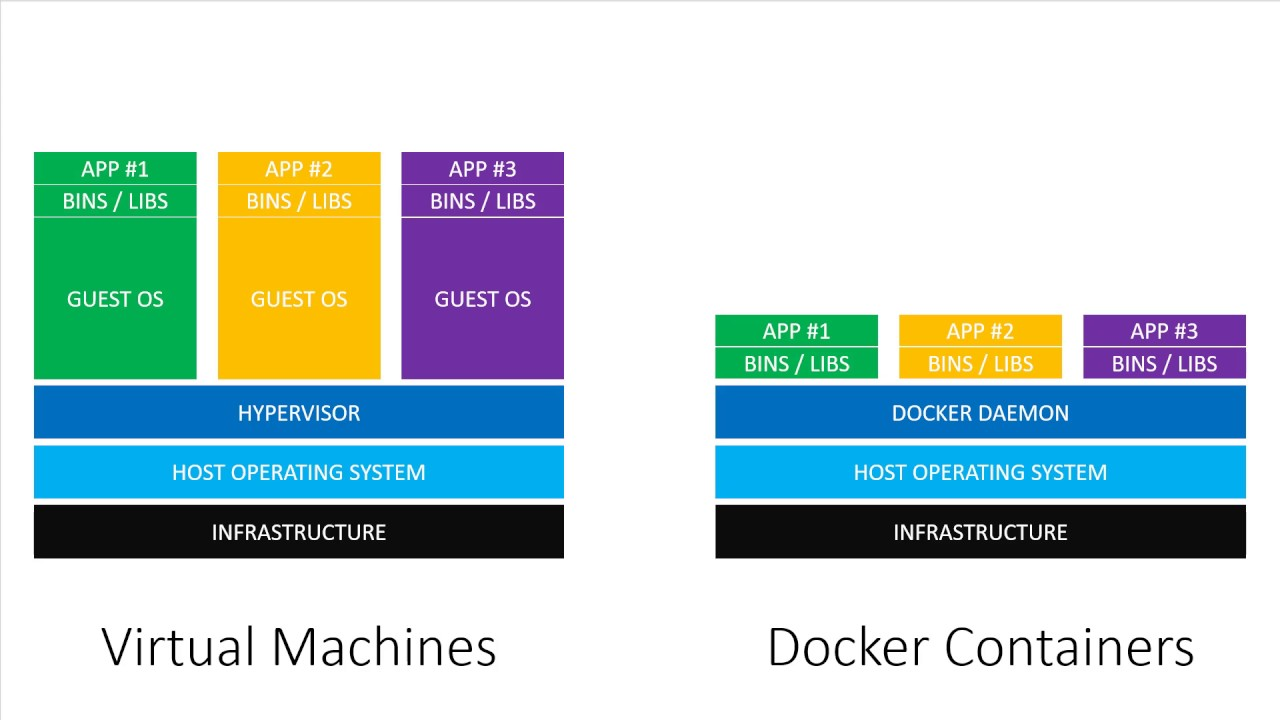
\includegraphics{img/vmvsdocker.jpg}

\end{frame}

\begin{frame}

Os pricipais conceitos do \emph{Docker} são:

\begin{itemize}
\item
  \textbf{Imagens}: instruções de como construir os containers
\item
  \textbf{\emph{Containers}}: as ``máquinas virtuais'' já construídas a
  partir dos containers
\item
  \textbf{Volumes}: pastas no computador hospedeiro que o container irá
  utilizar para armazenar arquivos permanentemente
\item ~
  \hypertarget{redes-as-sub-redes-das-quais-os-containers-farao-parte}{%
  \subsection{\texorpdfstring{\textbf{Redes}: as sub-redes das quais os
  containers farão
  parte}{Redes: as sub-redes das quais os containers farão parte}}\label{redes-as-sub-redes-das-quais-os-containers-farao-parte}}
\end{itemize}

\end{frame}

\begin{frame}{Imagens}
\protect\hypertarget{imagens}{}

São as ``plantas'' que serão utilizadas para construir os
\emph{containers}

\end{frame}

\begin{frame}

São contruídas a partir de outras imagens que estão disponíveis no
repositório público do Docker (entitulado
\href{http://hub.docker.com}{Docker Hub})

\end{frame}

\begin{frame}

\begin{block}{Imagens de sistemas operacionais ``puros''}

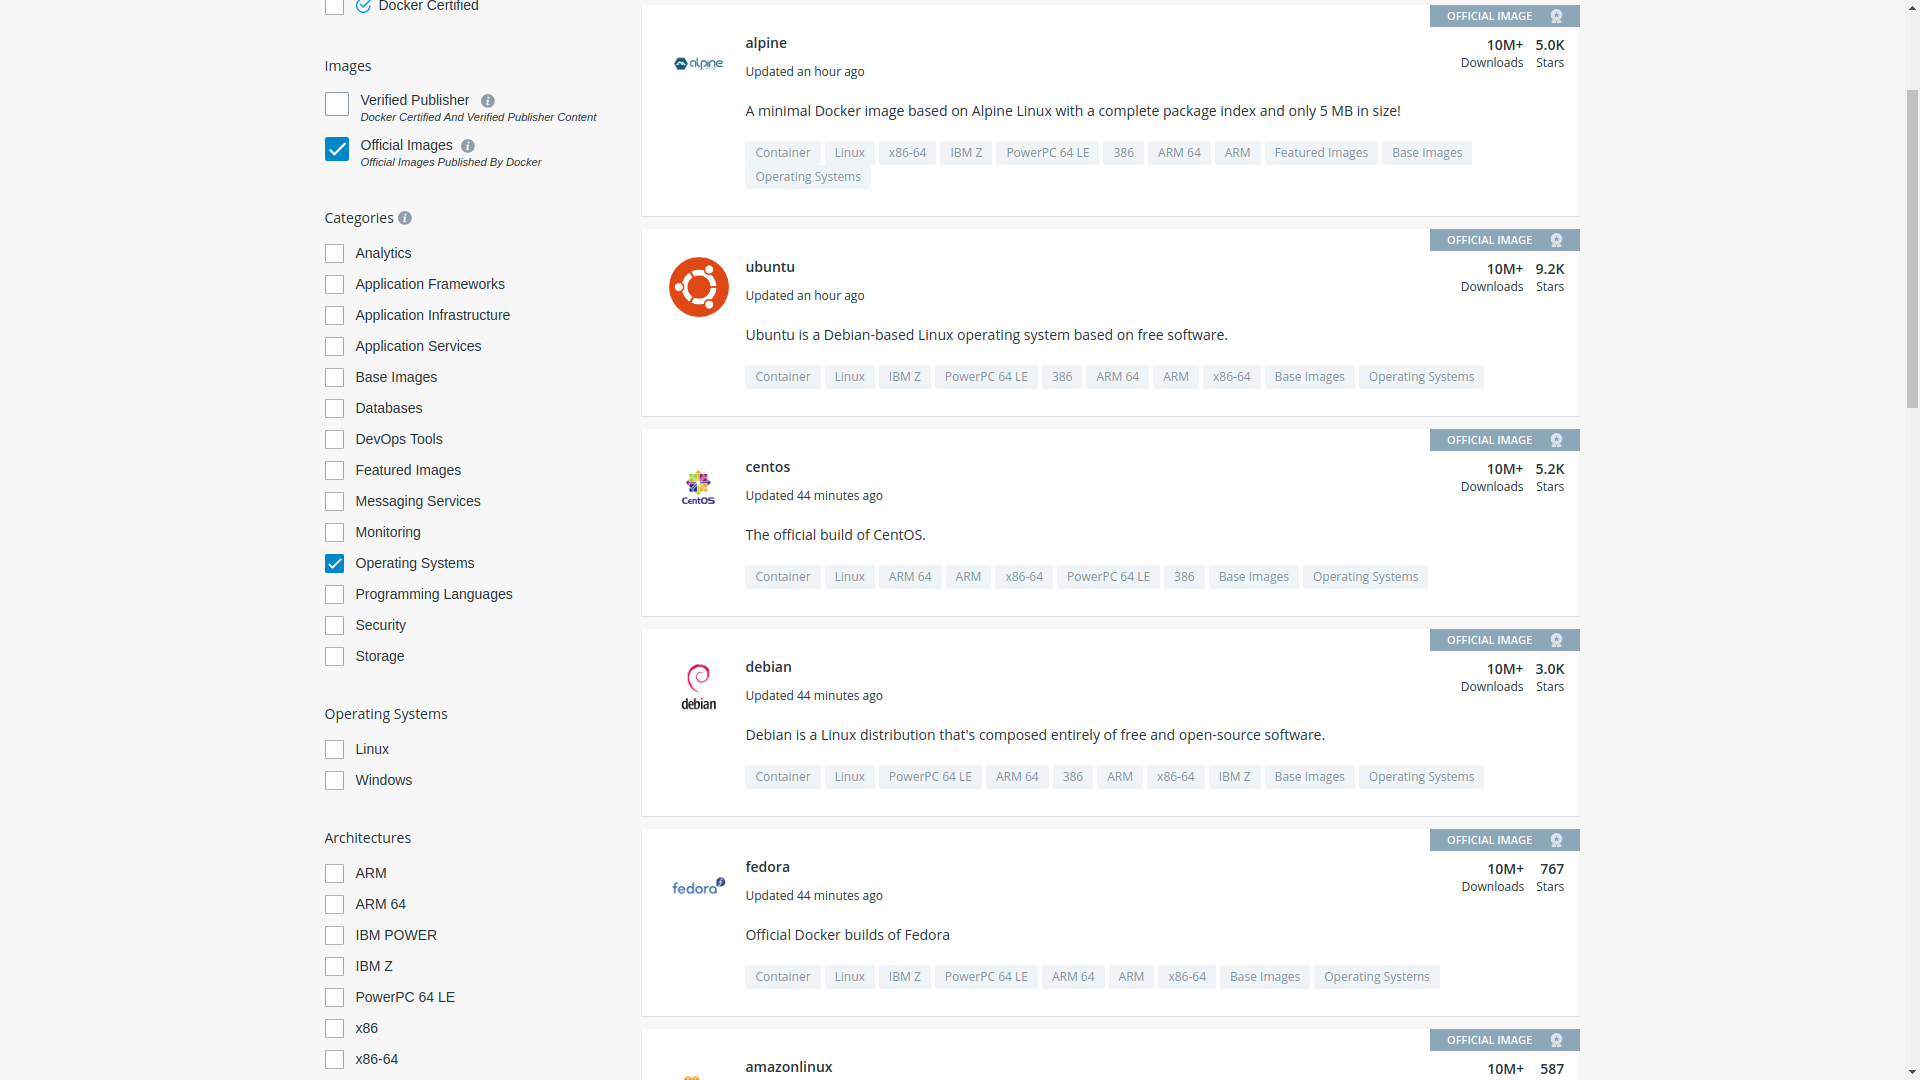
\includegraphics{img/hub-os.png}

\end{block}

\end{frame}

\begin{frame}

\begin{block}{Imagens de sistemas operacionais com linguagens
pré-instaladas}

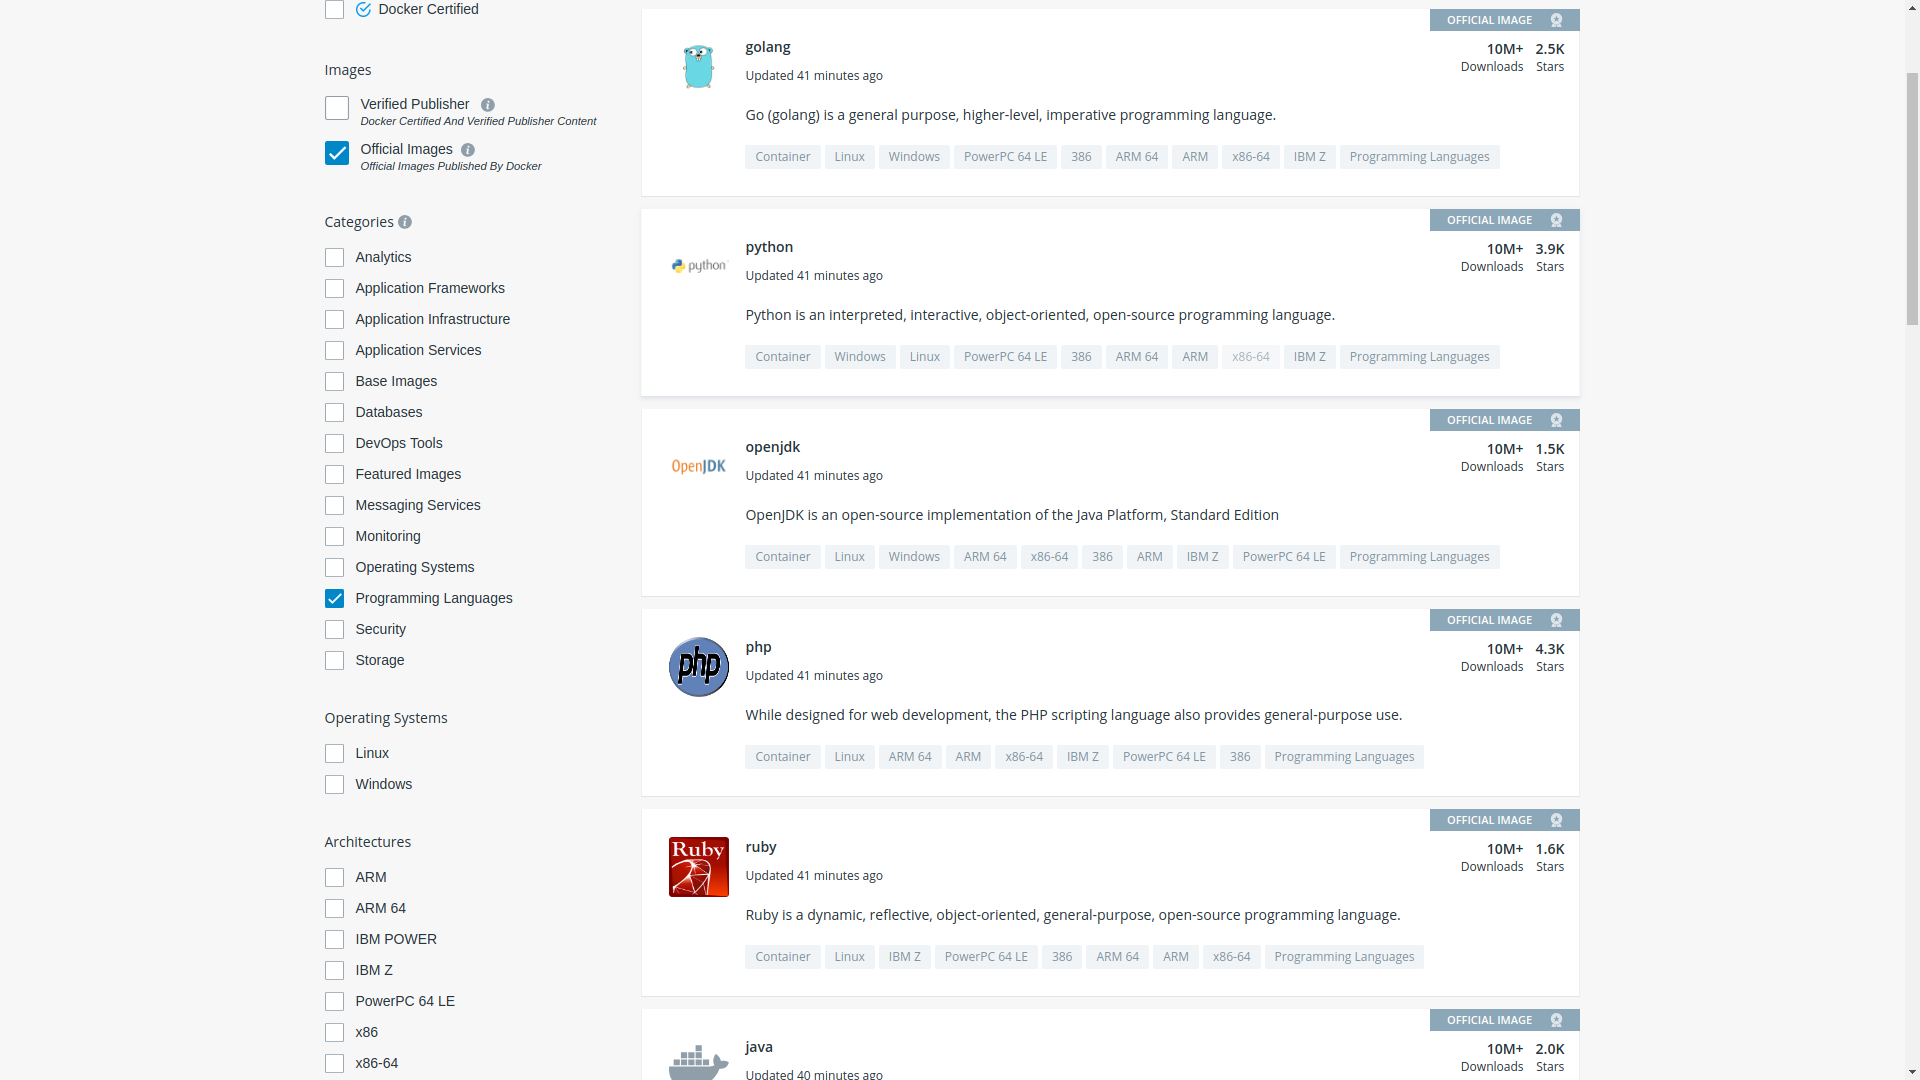
\includegraphics{img/hub-languages.png}

\end{block}

\end{frame}

\begin{frame}

\begin{block}{Imagens de sistemas operacionais com bancos de dados
pré-instalados}

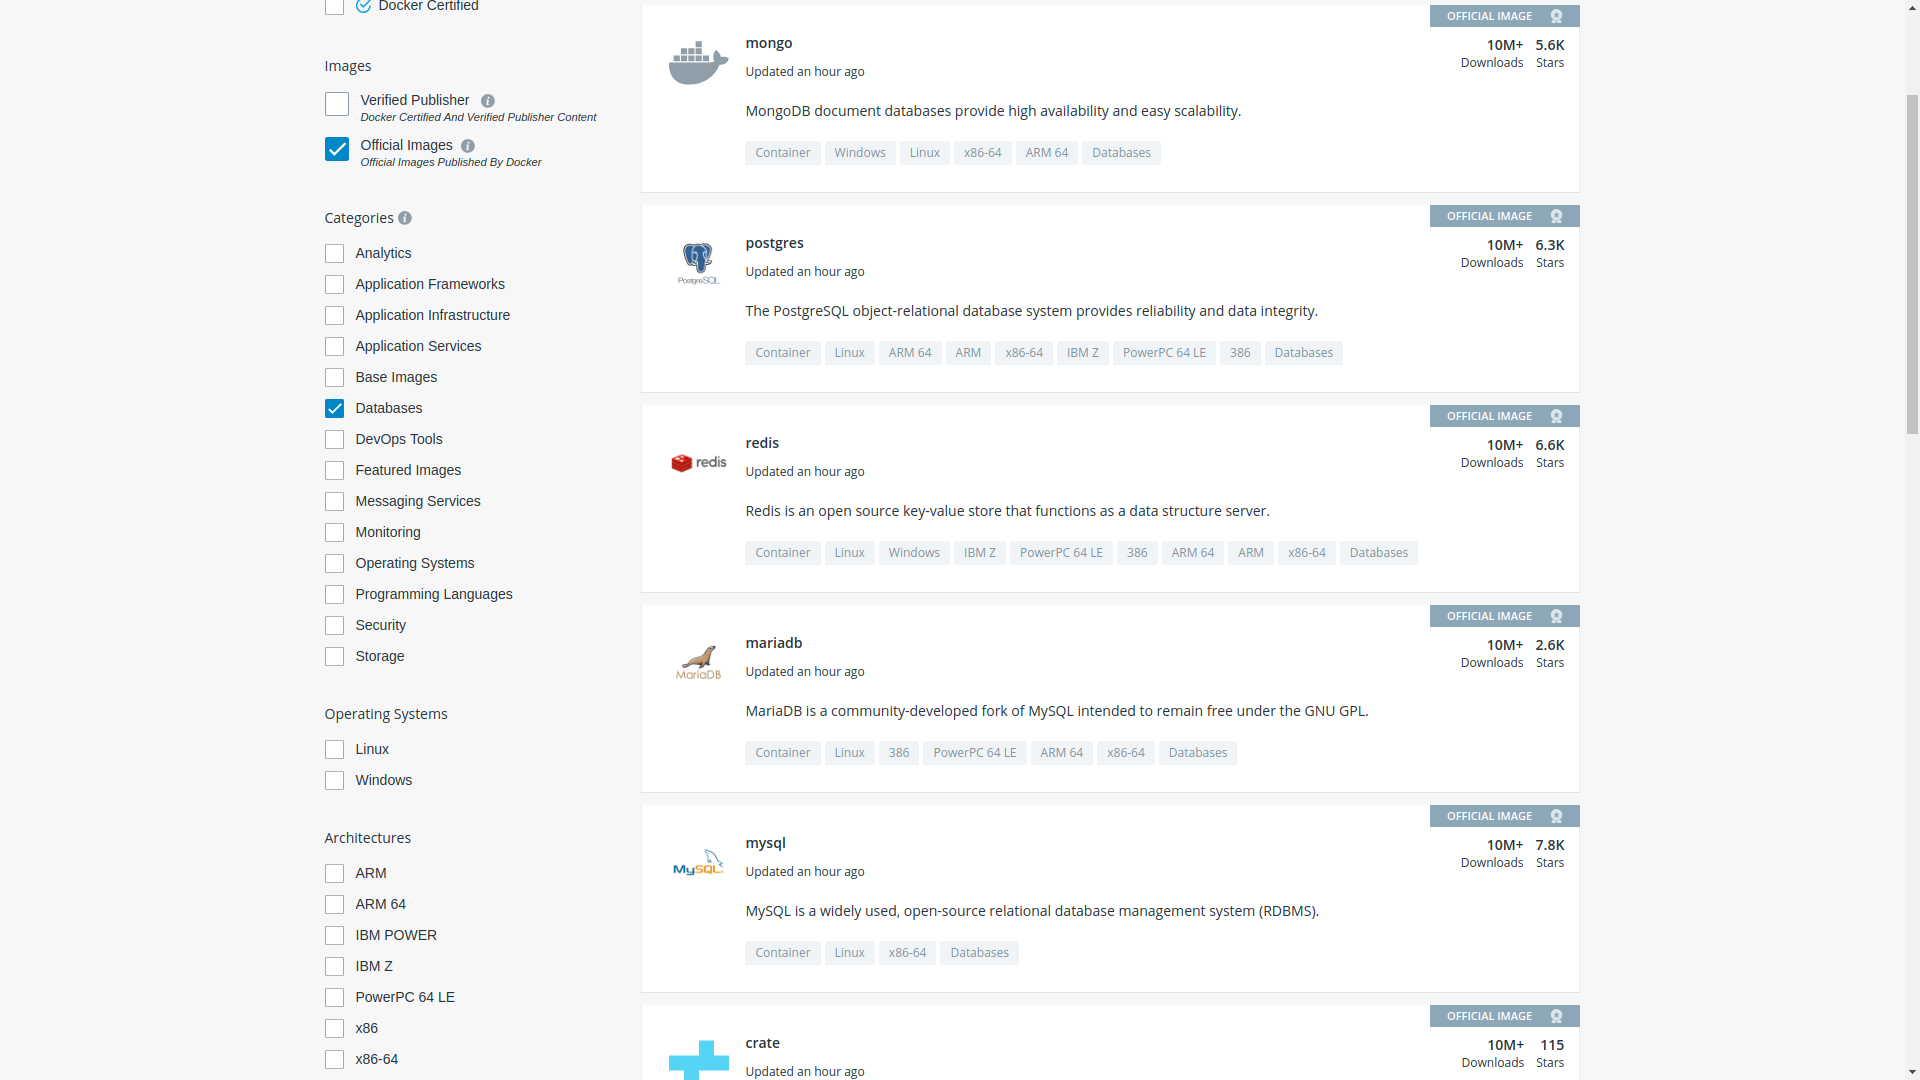
\includegraphics{img/hub-db.png}

\end{block}

\end{frame}

\begin{frame}

Ex: Se eu quiser construir uma imagem para um continer Linux que irá
fazer \emph{webscrapping} utilizando Celery eu posso criar a imagem:

\begin{itemize}
\tightlist
\item
  A partir da imagem de um Linux puro (Alpine, Ubuntu etc)
\item
  A partir da imagem oficial do Python (que por sua vez foi criada a
  partir da imagem de um Linux puro)
\item
  A partir de uma imagem que já tenha Celery instalado e configurado
\end{itemize}

\end{frame}

\begin{frame}[fragile]

Trechos do \texttt{Dockerfile} do \emph{MySQL}

\end{frame}

\begin{frame}[fragile]

\begin{Shaded}
\begin{Highlighting}[]
\CommentTok{# Usando outra imagem como ponto de partida}
\ExtensionTok{FROM}\NormalTok{ debian:stretch-slim }\CommentTok{# ...}
\CommentTok{# Executando comandos para instalar pacotes}
\ExtensionTok{RUN}\NormalTok{ apt-get update }\KeywordTok{&&} \CommentTok{# ...}
\CommentTok{# Definindo variáveis de ambiente}
\ExtensionTok{ENV}\NormalTok{ GOSU_VERSION 1.7 }\CommentTok{# ...}
\CommentTok{# Expondo uma das pastas para o hospedeiro}
\ExtensionTok{VOLUME}\NormalTok{ /var/lib/mysql }\CommentTok{# ...}
\CommentTok{# Copiando arquivos para a imagem}
\ExtensionTok{COPY}\NormalTok{ config/ /etc/mysql/ }\CommentTok{# ...}
\CommentTok{# Expondo a porta 3306 para o hospedeiro}
\ExtensionTok{EXPOSE}\NormalTok{ 3306 33060 }\CommentTok{# ...}
\CommentTok{# Executando o deamon do MySQL}
\ExtensionTok{CMD}\NormalTok{ [}\StringTok{"mysqld"}\NormalTok{]}
\end{Highlighting}
\end{Shaded}

Fonte:
\href{https://github.com/docker-library/mysql/blob/a7a737f1eb44db467c85c8229df9d886dd63460e/8.0/Dockerfile}{MySQL
Docker File}

\end{frame}

\begin{frame}

Esses comandos serão executados toda vez que um novo container de MySQL
for construído.

\end{frame}

\begin{frame}

Observações importante: \textbf{o sistema de arquivo dos
\emph{containers} é volátil!}

(Isso ficará mais claro quando falarmos sobre volumes)

\end{frame}

\begin{frame}{\emph{Containers}}
\protect\hypertarget{containers}{}

\emph{Containers} são instâncias de imagens.

\end{frame}

\begin{frame}

\begin{itemize}
\tightlist
\item
  Um \emph{container} é gerado a partir de uma imagem
\item
  Um hospedeiro pode executar vários \emph{containers} simultaneamente
\end{itemize}

\end{frame}

\begin{frame}

Analogia: a imagem é o molde e os \emph{containers} são os objetos
criados a partir desse molde

\end{frame}

\begin{frame}

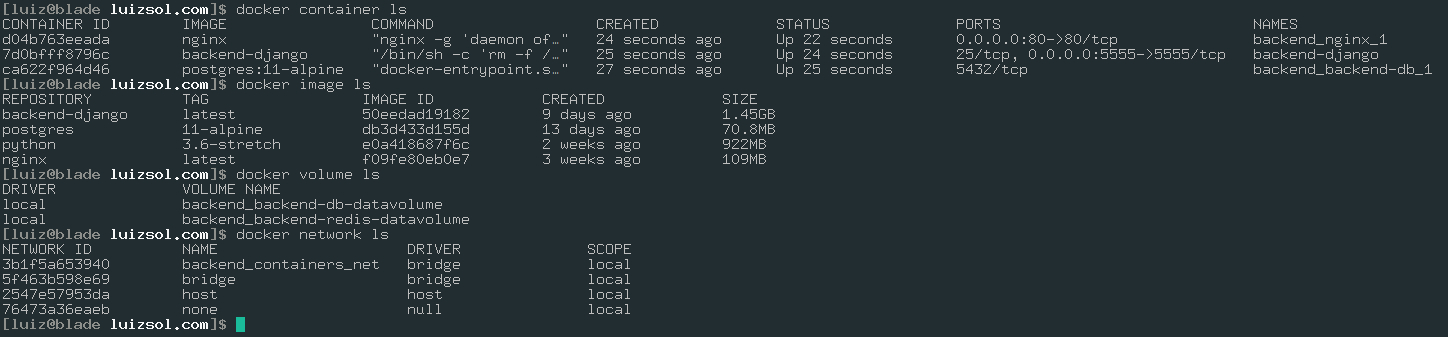
\includegraphics{img/containers.jpg}

\end{frame}

\begin{frame}

teste

\end{frame}

\end{document}
